\documentclass[tikz,border=1mm]{standalone}
\usepackage{tikz}
\usepackage{pgfplots}
\pgfplotsset{compat=1.18}
\usepackage{amsmath}

\begin{document}

% f1(t) = 1

\begin{tikzpicture}
\begin{axis}[
    scale=0.6,
    ytick=1,
    xtick=1,
    axis lines=middle,
    xmin=0, xmax=1.1,
    ymin=0, ymax=1.1,
    samples=2,
    domain=0:1]
\addplot[blue,thick]{1};
\end{axis}
\end{tikzpicture}


% f2(t) = t

\begin{tikzpicture}
\begin{axis}[
    scale=0.6,
    ytick=1,
    xtick={1},
    axis lines=middle,
    xmin=0, xmax=1.1,
    ymin=0, ymax=1.1,
    samples=2,
    domain=0:1
]
\addplot[blue, thick] {x};
\end{axis}
\end{tikzpicture}


% f3(t)

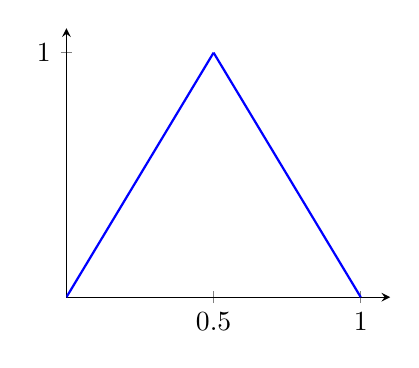
\begin{tikzpicture}
\begin{axis}[
    scale=0.6,
    ytick=1,
    xtick={0.5,1},
    axis lines=middle,
    xmin=0, xmax=1.1,
    ymin=0, ymax=1.1,
    samples=2,
    domain=0:1
]
\addplot[blue, thick, domain=0:0.5] {2*x};
\addplot[blue, thick, domain=0.5:1] {2-2*x};
\end{axis}
\end{tikzpicture}


% f4(t)

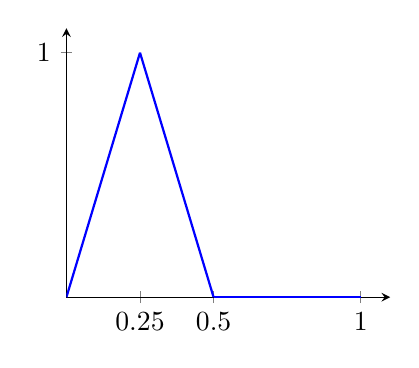
\begin{tikzpicture}
\begin{axis}[
    scale=0.6,
    ytick=1,
    xtick={0.25,0.5,1},
    axis lines=middle,
    xmin=0, xmax=1.1,
    ymin=0, ymax=1.1,
    samples=2,
    domain=0:1
]
\addplot[blue, thick, domain=0:0.25] {4*x};
\addplot[blue, thick, domain=0.25:0.5] {2-4*x};  % equivale a -3x
\addplot[blue, thick, domain=0.5:1] {0};
\end{axis}
\end{tikzpicture}


% f5(t)

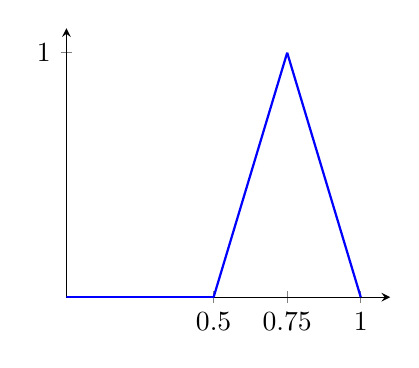
\begin{tikzpicture}
\begin{axis}[
    scale=0.6,
    ytick=1,
    xtick={0.5,0.75,1},
    axis lines=middle,
    xmin=0, xmax=1.1,
    ymin=0, ymax=1.1,
    samples=2,
    domain=0:1
]
\addplot[blue, thick, domain=0:0.5] {0};
\addplot[blue, thick, domain=0.5:0.75] {4*x-2};
\addplot[blue, thick, domain=0.75:1] {4-4*x};
\end{axis}
\end{tikzpicture}

\end{document}